\chapter{Solar irradiance simulation tools}
The primary tool used in this thesis for simulating PV generation with different parameters is the python library PVlib. PVlib contains be built functions for estimating solar irradiance, angle of incidence and a multitude of other useful tools. As seen from table \ref{table_poa_simulated_format}, the plane of array(POA) simulations which estimate the irradiance per 1m² of solar panel surface resemble the earlier FMI PV datasets in their structure.

%An example of the irradiance simulation outputs is shown in table \ref{table_poa_simulated_format} and the table shows that the output format is simular to the FMI PV datasets shown earlier in table \ref{table_fmi_kumpula_csv}.




%Having a mathematical model which would simulate the output of a PV system would allow for the parameters of a PV installation to be solved with model fitting. In the best case scenario, we would have a physics based model which would take geographic location, panel installation angles, time of year and panel surface area or power rating as inputs and the output would be similar to the data from FMI Kumpula installation seen in table \ref{table_fmi_kumpula_csv}. Creating a such model is rather challenging as the model has to take into account atmospheric scattering, Sun angles, Sun-Earth distance variation and a multitude of other factors, the consideration of which are far beyond this mathematics thesis. Luckily the modeling of the energy output of solar PV installations has uses for the cost-benefit analysis of solar PV installations and thus pre-existing modeling algorithms are publicly available. 


% TODO REWRITE

%This thesis uses a plane of array irradiance simulation function from the python library PVlib. The function takes geographic location, timestamp and panel angles as inputs. The outputs contain power values which describe the amount of direct and atmospherically scattered light that would hit a square meter sized imaginary solar panel with the input parameters. The sum of these sources is referred as plane of array (POA) irradiance and this value can be used to estimate the output of solar power installations. A section of simulated data is included in table \ref{table_poa_simulated_format}.

%As the model simulates radiation values during clear sky conditions and not the power output of pv installations, the model should be seen as an approximation which is accurate to a certain degree. The differences between the model and recorded measurements could be due to reflectivity of the solar panels, weather conditions, temperature related changes in efficiency, atmospheric composition or a multitude of other factors which the model does not take into account.

\begin{table}[h]

\centering

\begin{tabular}{r|cccc} \hline\hline

Timestamp[UTC] & Minute & POA(W) \\ \hline
$2018-05-30$ $00:00$ &  $0$ & $0.0$\\
$2018-05-30$ $00:01$ &  $1$ & $0.0$\\
$2018-05-30$ $00:02$ &  $2$ & $0.0$\\
\vdots & \vdots & \vdots \\
$2018-05-30$ $ 07:34$ & $454$ & $800.691861$\\
$2018-05-30 $ $07:35$ & $455$ & $802.110516$\\
$2018-05-30 $ $07:36$ & $456$ & $803.517424$\\
\vdots & \vdots & \vdots \\
$2018-05-30$ $ 23:57$ & $1437$ & $0.0$\\
$2018-05-30 $ $23:58$ & $1438$ & $0.0$\\
$2018-05-30 $ $23:59$ & $1439$ & $0.0$\\

\hline\hline
\end{tabular}
\tabcaption{One day of simulated plane of array irradiance values. Note that the minute column is added to the table for convinience and it is reduntant as minutes can be read from the timestamps.}
\label{table_poa_simulated_format}
\end{table}

%\section{PVlib POA python function} % , parameter space and computational requirements}
%Taking a look at the code responsible for the plane of array irradiance simulations can give some insights into the behavior of the estimations and problem of parameter estimation. The  python function responsible for simulating plane of array irradiance values over a day is defined with the header \ref{poa_header}. In this header we can see that the function takes 7 inputs each of which is mandatory, meaning that when the functions is used as a tool for parameter estimation, some of the parameters have to be guessed or randomly assigned.

%\begin{lstlisting}[caption={PVlib POA simulation function header.}, label={poa_header}]
%def get_irradiance_with_multiplier(year, day, latitude, longitude, tilt, azimuth, multiplier):
%\end{lstlisting}







%The following python code is a function which adds the ability to scale the power values of PVlib POA simulations. This ability is needed as by default PVlib simulates the amount of energy radiated towards an imaginary square meter sized solar panel with given coordinates, timestamp and installation angles and as such the power values have to be scaled in order to match the surface areas and efficiency of real installations. The code itself does not tell much of the mathematics used for the simulation, but it can be used to show the input parameters required by the POA simulation function. Each of the 6 parameters is mandatory, meaning that if latitude, longitude, day or any other parameter is left out when the function is called, this will raise an error upon code execution. This means that when the functions is used as a tool for parameter estimation, some of the parameters have to be guessed or randomly assigned. 

%This wrapper shows that six input variables are used for generating a day long POA simulation. The functions requires these parameters, meaning that python will raise an error if the function is called without the necessary 6 inputs. This means that when the function $get\_irradiance\_with\_multiplier()$ is used as a tool to solve the parameters of a system, up to 5 parameters may have to be guessed or assigned random values. The parameters and their ranges are as follows:
\subsection{Python function and input parameters} 
In the thesis code, the irradiance simulation function is declared with the following function header.

\begin{lstlisting}[caption={PVlib POA simulation function header.}, label={poa_header}]
def get_irradiance(year, day, lattitude, longitude, tilt, azimuth):
\end{lstlisting}


\noindent The following listing contains the parameters of the plane of array irradiance function and their domains.
%The POA simulation function accepts real --or integer as is the case with the day parameter-- valued parameters in the ranges listed below. 

\begin{itemize}
	\item Year $\in \mathbb{N}$
	\item Day [1, 365/366] $\in \mathbb{N}$
	\item Latitude [-90, 90] $\in \mathbb{R}$%, Finland fits within subrange [59, 70]
	\item Longitude [-180, 180]  $\in \mathbb{R}$%, Finland fits within subrange [19, 32] 
  	\item Tilt [0, 90] $\in \mathbb{R}$
  	\item Azimuth [0, 360[ $\in \mathbb{R}$
\end{itemize}

%\noindent \textbf{Note:} While the function does accept the full latitude and longitude ranges as inputs, it may be beneficial to restrict the range of the coordinate parameters when the approximate location of the installation is known. For example, Finland fits within subrange [19, 32] on the longitude axis and thus it could make sense to restrict the longitude range when examining installations located within Finland.

\vspace{3mm}
\noindent
The day and year parameters can be assumed to be always known and this leaves four unknown system parameters. If each parameter combination results in an unique output, the likely system parameters can be solved by exhaustively searching the parameter space and comparing the resulting output data to known power generation data.

The combination of these four parameters and their ranges can be thought to form a subspace in four-dimensional Euclidean space. This so-called parameter space and its "volume" are both concepts that can be used for analyzing the difficulty of parameter estimation problems, behavior of parameter estimation functions and their efficiency. In general, the more parameters and thus dimensions there are, the larger the resulting parameter space is and the harder the problem becomes. And the more parameters an algorithm is attempting to solve at once, the slower the algorithm can be expected to be. If each parameter is discretized to 20 evenly spaced values, solving all the 4 parameters at once by testing out every possible combination would require evaluating $20^4$ or 160 000 unique combinations. However if the parameters could be solved one by one, isolted from the influence of other parameters, there would only be $20*4$ or 80 unique combinations, a reduction of 2000 to 1. This highlights how important it is to break larger problems into smaller problems whenever possible.



%\noindent The combination of these parameters and their ranges can be thought to form a subspace in seven-dimensional Euclidean space, or six dimensional if year and day are combined into a date variable. This so-called parameter space and its "volume" are both concepts that can be used for analyzing the difficulty of parameter estimation problems, behavior of parameter estimation functions and their efficiency. In general, the more parameters and thus dimensions there are, the larger the resulting parameter space is and the harder the problem becomes. And the more parameters an algorithm is attempting to solve at once, the slower the algorithm can be expected to be.

%With solar PV installation parameter estimation, there are 5 unknown parameters as the year and day parameters are always known. If each of the remaining parameters is discretized to 20 evenly spaced values, solving all the 5 parameters at once by testing out every possible combination would require evaluating $20^5$ or 3.2 million unique combinations. However if the parameters could be solved one by one, isolted from the influence of other parameters, there would only be $20*5$ or 100 unique combinations, a reduction of 32000 to 1. This highlights how important it is to break larger problems into smaller problems whenever possible.

%In the worst case where none of the 6 parameters are known and each of the parameter space axes are discretized to $n$ unique evenly spaced values, then the amount of possible combinations is $n^6$. 

%The exponent of 6 may seem insignificant, but even with a crude space discretization where $n$ is chosen to be 20 would result in 64 million combinations. If testing out one parameter combination were to take a second of computing time, testing out each of the 64 million combinations would require more than 700 days of non-stop computing. Luckily the day parameter is always known and thus $n^6$ drops into $n^5$ but even then the size of the parameter space is enormous.

%Thus the goal of the parameter estimation functions should be to reduce the freedom of movement in the parameter space as efficiently as possible, eventually restricting the parameter space into an individual point which corresponds to the installation parameters of the system.


%This means that when unknown parameters of a multi parameter function are being solved, emphasis should be placed on solving the parameters one by one


%In best case scenario, one or more of these parameters can be locked to a specific value. This decreases the volume of the parameter space and the goal 


%the amount of different parameter combinations that may have to be tested while the installation parameters are being solved. 



%The amount of dimensions is relevant as if $n$ discrete values are chosen for each parameter, the total amount of different parameter combinations would be $n^6$. Luckily the day parameter is always known and thus there are only 5 free dimensions, but this still results in a fairly large parameter space. Even a crude discretization with 20 values per dimension would still result in $20^5$ or 3.2 million different parameter combinations. 

%The amount of parameter combinations is relevant as some problems may prove to be difficult to solve intelligently. In these cases, testing out every parameter combination may be the only option. However exhausting the parameter space may not be viable if the space is extremely large.


%With extremely large parameter spaces even this method may become unviable as the computing time and energy required 




%In theory, if we could design a function which could determine if the POA simulation and the real world measurements match, then it would be possible to test out every possible parameter combination until the correct set of parameters was found. In practice however, this would not be adviseable or in some cases even possible as the parameter space is enormous. In the case where the range of each parameter was split into equidistant points, each of which had to be tested for, in total there would be $20^5$ or 3.2 million different sets of parameters. If testing out one set of parameters would take about a second of computing time, then the complete set of 3.2 million unique parameter combinations would require almost 40 days of non stop computations.




%The following python code generates a scaled POA curve for a day of data with given input parameters. As the code is a wrapper for the more complex $get\_irradiance$ fuction, it can be written with just a few lines of code and it should highlight the parameters used by the PVlib simulation function. The 6 necessary parameters are latitude, longitude, day, tilt, facing(azimuth) and multiplier. This means that the parameter space of the POA model is a 6 component vector. Luckily the day can be assumed to be always known and as such there are only 5 unknown parameters which span the parameter space.


%def get_irradiance(lat, lon, day, tilt, facing):

%This thesis uses a plane of array irradiance simulation function from the python library pvlib to simulate the energy output of solar pv installations. The inputs of said function are the geographic location of the installation, timestamp and panel installation angles. And the output of the function is a python pandas dataframe, a table-like entity with timestamps as indices and watts per square meter as the indexed data. 



%According to the PVlib documentation, the plane of array irradiance function returns multiple different power values. Out of these the "poa_global" is a watts per square meter estimation of the direct and indirect diffuse light that would hit a solar panel with the given coordinates, date and panel angles. A such model 

% https://pvlib-python.readthedocs.io/en/v0.9.0/generated/pvlib.irradiance.poa_components.html



%describes the amount of direct and indirect radiation which would hit the surface of a solar panel at given coordiantes, date and panel angles. Note that it does not take into account the reflectivity of the panels, efficiency loss due to heat or a multitude of other factors and the lack of these features will introduce some errors in the results. 
 
% TODO REWRITE END

%In addition, the pvlib poa function included in the appendix \ref{pvlib_poa_code} does not take into account the panel surface area and thus an additional function \ref{pvlib_poa_multiplier_code} was written. And unless otherwise denoted, the POA function \ref{pvlib_poa_code} will be assumed to be a black box function, meaning that the exact behavior of the pvlib function is expected to be unknown.

\newpage
\section{PVlib POA evaluation}

Before implementing the parameter estimation functions, the POA simulations should be tested against known measurement data. Figure \ref{fig-multidaypoavsmeasurements} indicates that in clear sky conditions the pvlib irradiance model is following real world measurements closely with a few exceptions. During cloudy days, the measurements can be seen to exceed the power generation estimated by the model. The cause for this increase is likely to be caused by the additional sunlight reflected from clouds towards solar panels in partly cloudy weather conditions and it shows that cloud induced noise can be positive as well as negative. 

%There is also some deviation visible in the power values of first and last non-zero hours which may prove to be an issue in later stages.

%The same figure shows the importance of finding clear sky days as the only charasteristic in the measurement plots which seems to be consistent between the cloud free and cloudy days seems to the timing of the first and last non-zero minutes. In the 240th day for example, most of the measurements are either higher or lower than the estimated values, but the first and last non-zero minutes seem to align with the first and last non-zero minutes of POA simulations. On the 70th and 150th day, the difference between the modeled and measured first and last non-zero minutes is visible on the graph. Whether this difference is significant will depend on the algorithms applied.

% Proper evaluation of the irradiance model is not the topic of the thesis and as such 

\begin{figure}[h]
\centering
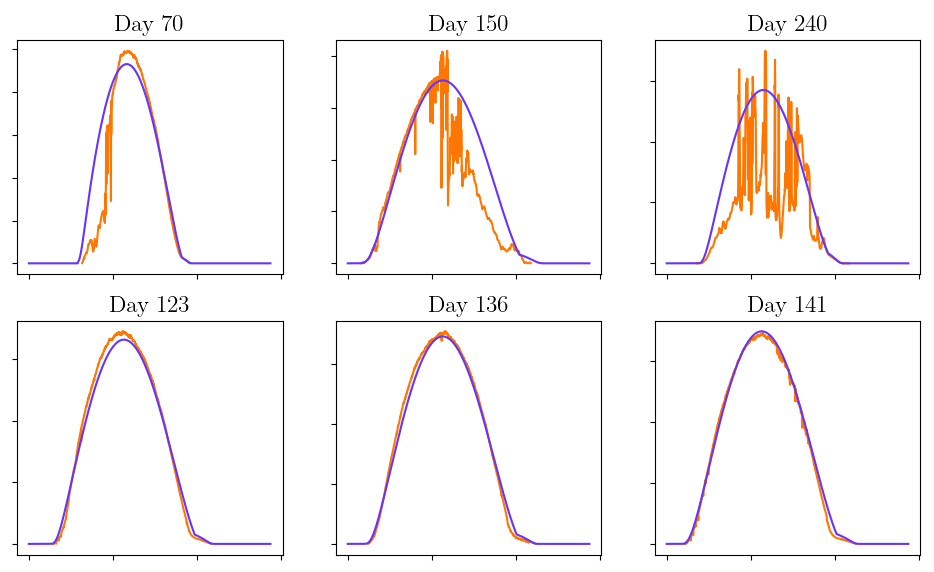
\includegraphics[width=1\linewidth]{pics/multiday_vs_neat}
\figcaption{Power output of FMI Kumpula PV installation and the pvlib POA simulation computed with the parameters \ref{table_fmi_helsinki_kuopio_parameters}. Horizontal axis on the graphs corresponds to time and vertical axis marks the estimated power values. The purpose of the graphs is to display the different shapes and deviations from POA models and thus axis names and numbers were left out. Upper row contains randomly selected days while as the lower row has days chosen by a clear sky algorithm mentioned in chapter \ref{clearskyalgo_chapter}. Measurements are from 2017. POA irradiance values were multiplied by 20 in order to match the curves values on power axis.}
\label{fig-multidaypoavsmeasurements}
\end{figure}



% On the 70th and 150th day, the first and last minutes do not seem to be exactly the same as in the simulation, but the difference seems minor and it is occuring in different directions.






%\textit{The following claims are unverified conjectures, but the smooth shape and the early date of the first graph could hint that the increased peak production on the 70th day could be due to reflections from snow, while as the more irregular production on the 150th and 240th day would seem to indicate that the variation is caused by clouds. Filtering out days such as the 150th or the 240th from the dataset should be rather simple as the high frequency component is noticeable, but low frequency deviations such as the smooth increase in production of the 70th day could prove to be more difficult to detect algorithmicly.}






\newpage
%\section{Influence of different parameters on the PVlib poa model}
%\label{influence_parameters}



\begin{figure}[ht!]
\centering
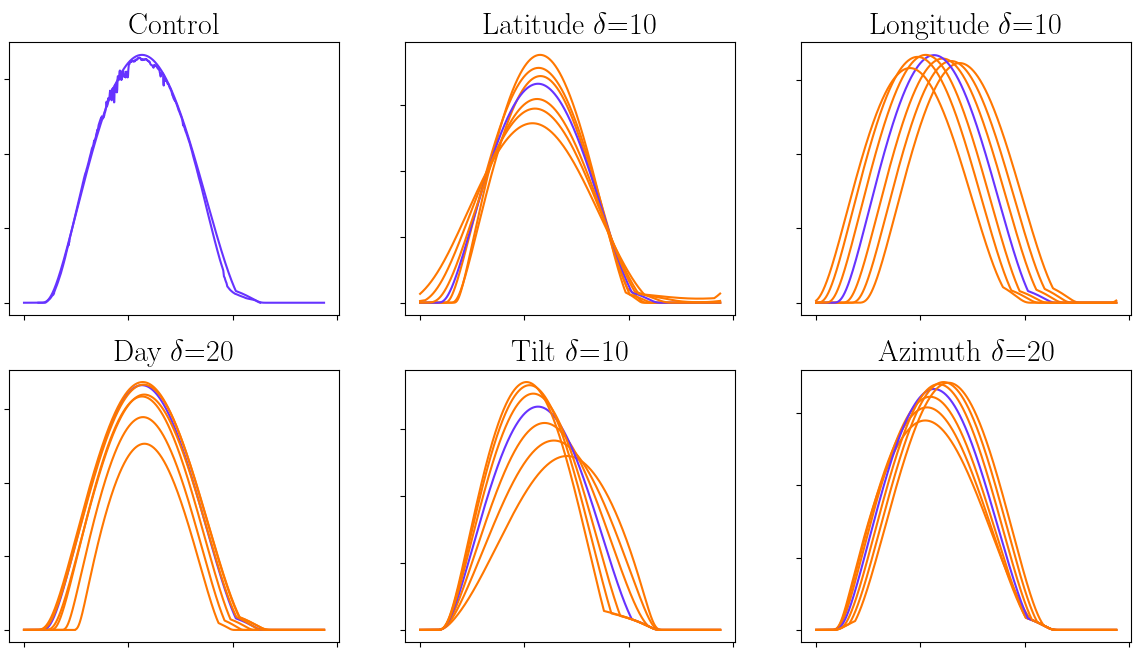
\includegraphics[width=0.8\linewidth]{pics/poa_eval_new_crop}
\figcaption{Influence of changes in PVlib simulation parameters on generated power output curves. Control shows FMI Helsinki measurements and simulation with the same parameters as the Helsinki installation. Simulated power values are multiplied by 19 in order to match values on y-axis.}
\label{fig_poa_different_parameters}
\end{figure}

By varying the different simulation parameters as shown in figure \ref{fig_poa_different_parameters}, we can examine the relationships between parameters and power generation curves. This can help us understand if there are usable patterns in the data. In the best case scenario each of the simulation function inputs would affect one measureable property in the irradiance plots and their relationship would be bijective. To give an example, if the peak power minute was isolated from all other parameters than the longitude and the relationship between longitude and peak power minute was linear, it would be possible to solve the peak power minute to longitude function with just a few plane of array irradiance simulations.

In the exact opposite case where every measureable property of irradiance plots is affected by every input parameter, solving the parameters would be much harder or even impossible. For example if all of the parameters influenced the same traits to different extents and the system was not bijective, multiple parameter combinations could result in the same simulated power graph. In a such system there would not be a single solution but rather a set of possible solutions.

The problem of solving installation parameters lies somewhere in between the two extremes. The longitude parameter would seem to shift the curve along the time axis where as tilt and azimuth parameters do not affect the first or last non-zero minutes but they do affect the shape of the curve. Observations of parameter to trait interactions are listed on table \ref{table_traits}.



\begin{table}[H]
\centering
\begin{tabular}{r|cc} \hline\hline

 Parameter & Traits affected\\ \hline
 Latitude & Shape, first and last minute times\\
 Longitude & First and last minute times\\
 Tilt & Shape\\
 Azimuth & Shape\\

\hline\hline
\end{tabular}
\tabcaption{Function input to observed trait table.}
\label{table_traits}
\end{table}


%Base on these observations, the relationship between longitude and the First and last minute times would seem like the best starting point for parameter solving.

%If the POA model is assumed to be accurate, the model could be used to simulate the effects of different parameters on power generation. This could provide insights into the relationship between patterns in the data and the parameters of the system. The relevant parameters to simulate and their default values can be seen in table \ref{table_default_parameters_poa_simulations}. In the following simulations, only one of the default parameters is varied. This is done in order to isolate the effect of individual parameters.



%\begin{table}[!ht]
%\centering
%\begin{tabular}{r|c} \hline\hline

% Parameter & Value \\ \hline
% Day & $180$  \\
% Latitude & $60^\circ$  \\
% Longitude & $28^\circ$  \\
% Panel tilt & $30^\circ$ \\
% Panel angle & $180^\circ$  \\
%\hline\hline
%\end{tabular}
%\tabcaption{Default parameters for POA simulation used in this section. }
%\label{table_default_parameters_poa_simulations}
%\end{table}


\newpage

\subsection{Influence of different longitudes}
\label{section_different_longitudes}

\begin{figure}[ht!]
\centering
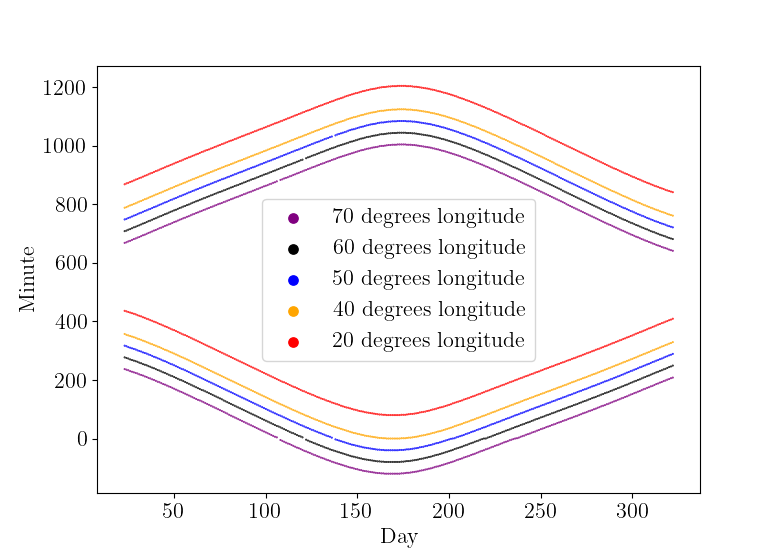
\includegraphics[width=1\linewidth]{pics/poa_var_lon}
\figcaption{First and last non-zero minutes of each day from year long simulations at different longitudes.}
\label{fig-poa_var_lon2}
\end{figure}

\noindent Based on earlier observations listed in table \ref{table_traits}, solving the longitude of installations would seem like a sensible starting point. The figure comparing the effects of different parameters seemed to suggest that the relationship between longitude and significant minute times is very close to linear and the same is seen here in figure \ref{fig-poa_var_lon2}. In Hagdadi 2017 \cite{navid_australian_article} and in Williams 2012 \cite{older_solar_solver_article} this relationship was used in order to determine the geographic longitude. The algorithms used by both of the articles relies on calculating an approximation for the time of the solar noon based on the average of the first and last minutes, this solar noon minute is then translated into a geographic longitude coordinate.





%There are at least two ways of estimating the longitude from the UTC solar noon time. First method is based on fitting a linear equation to a list of known solar noon to longitude-pairs. This would result in an equation of the form $f(x) = 0.25^\circ* x + b$ where the solar noon minute $x$ is multiplied by the constant $0.25$. The constant of $0.25^\circ$ comes from dividing a full circle by the amount of minutes in a day, 1440. The constant $b$ is around $-180^\circ$ and it is the result of solar noon occuring close to noon.
%In the figure \ref{fig-poa_var_lon2}, the relationship between the first and last minutes of a day and the geographic longitude can be seen to be linear. This linear equation should be of the form $f(x) = 0.25^\circ* x + b$ where the solar noon minute $x$ is multiplied by the constant $0.25$. The constant of$0.25^\circ$ comes from dividing a full circle by the amount of minutes in a day, 1440. The constant $b$ is roughly $-180$ degrees as that is the offset required for adjusting solar noon from



%and the figure \ref{fig-poa_var_lon2} it would seem that the relationship between longitudes and first and last minutes is a good starting point for parameter so


%at least very close to linear. In Hagdadi 2017 \cite{navid_australian_article} and in Williams 2012 \cite{older_solar_solver_article} this relationship was used in order to determine the geographic longitude. The algorithms used by both of the articles relies on calculating an approximation for the time of the solar noon based on the average of the first and last minutes, this solar noon minute is then translated into a geographic longitude coordinate.

% and a similar algorithm is detailed in []..




\newpage

\subsection{Influence of different latitudes}
\label{section_different_latitudes}

\begin{figure}[ht!]
\centering
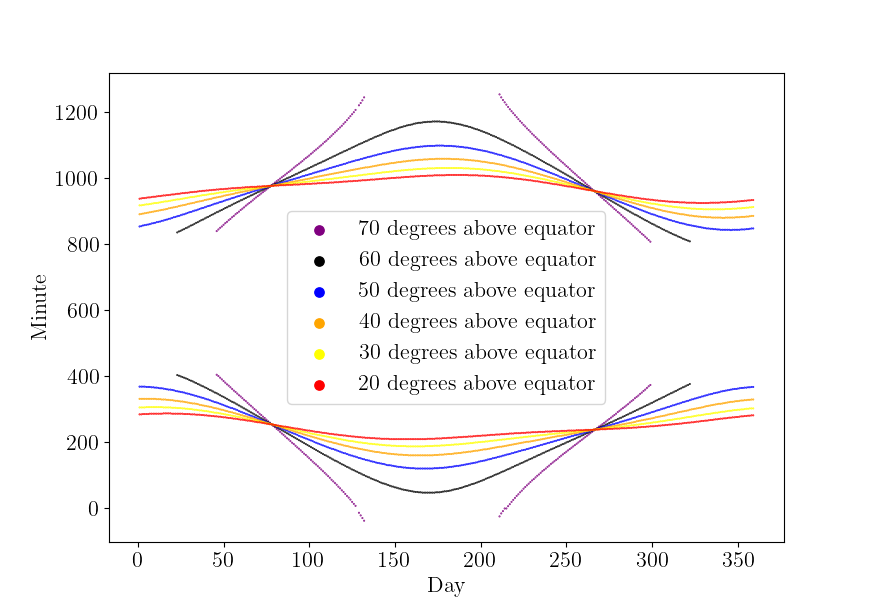
\includegraphics[width=1\linewidth]{pics/poa_var_lat}
\figcaption{First and last non-zero power minutes of each day from year long simulations at different latitudes}
\label{fig_poa_var_lat}
\end{figure}

\noindent The latitude simulations show that the day length stays fairly consistent for locations close to the equator, but with latitudes of $50^\circ$ and higher, the day to day variation is significant. These POA simulations would imply that the region around equinoxes is ideal for day length based analysis as there day length is always well defined and the rate of change can be measured. 


\newpage

\section{Increasing the accuracy of solar PV simulations}
\label{section_increased_accuracy_simulations}


\begin{figure}[h]
\centering
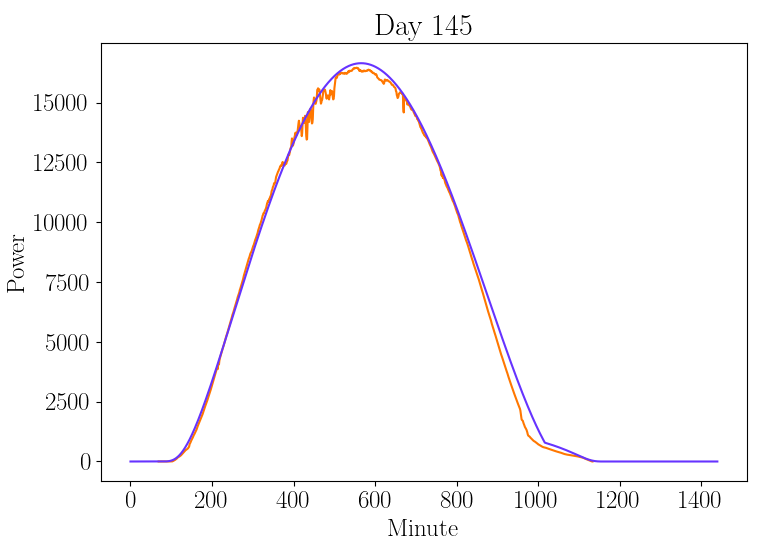
\includegraphics[width=0.7\linewidth]{pics/poa_eval_single_day}
\figcaption{Figure comparing Pvlib simulated POA irradiance and actual measured PV output of FMI Helsinki installation.}
\label{fig-poa_eval_single_day}
\end{figure}

\noindent Figure \ref{fig-poa_eval_single_day} compares the simulated and measured PV output during a sunny day in Helsinki. The shapes of the curves match quite closely, but there are some discrepancies. The estimated power values for the peak production hours are higher than measured power values and a similar phenomena is seen near minute 1000. These discrepancies can be explained by real world phenomena as PVlib POA values describe the amount of radiation reaching the surface of a solar panel. This is different from the power output of a PV system as thermal losses and panel reflections are not taken into account. This section examines an improved PV model which includes these losses.

\newpage

\subsection{Improved PV model}

\begin{figure}[h]
\centering
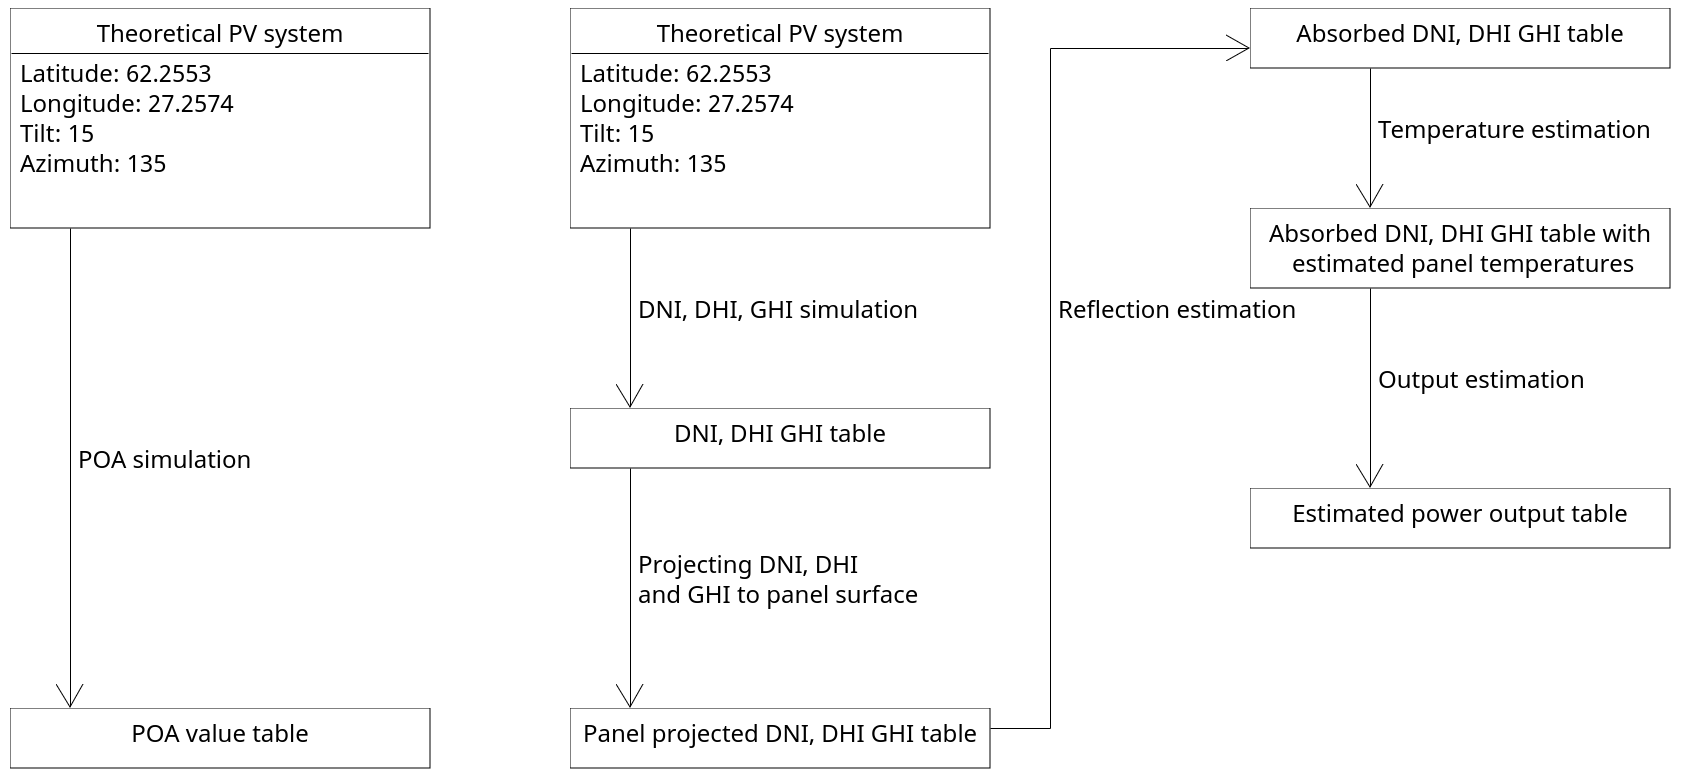
\includegraphics[width=1.0\linewidth]{pics/uml2}
\captionsetup{labelformat=empty}
\figcaption{Original POA-based PV model and the improved model with reflection and temperature estimation.}
\label{fig-pv_model}
\end{figure}


\noindent 
The improved PV model introduces some new concepts, the most important of which are the following irradiance types. 

\begin{itemize}
\item DNI is diffused normal irradiance which represents direct sunlight received by a 1m² -sized plane with AOI of 0 degrees. Note that athmosphere scattered or ground reflected irradiance are not components of DNI.

\item DHI is diffuse horizontal irradiance which represents the irradiance reaching a shaded 1m² -sized plane with tilt of 0 degrees. DHI represents atmosphere scattered irradiance.

\item GHI is global horizontal irradiance and it represents the amount of irradiance per 1m² -sized plane with tilt of 0 degrees. GHI is made up of direct irradiance and atmosphere scattered irradiance. GHI combined with albedo can be used to estimate the ground reflected irradiance.
\end{itemize}

\noindent
These irradiance types are present in both the simpler PVlib POA based model and the improved PV model. The difference between the two models is that in the POA-model, PVlib internally calculates three irradiance components DNI, DHI and GHI and projects them to the panel surface, returning this panel projected irradiance as plane of array irradiance. Where as in the more complex PV model, PVlib estimates DNI, DHI and GHI, each of which are processed by multiple functions before they are combined into an estimated power output value, resulting in a physically more accurate PV output estimation.

\subsection{Panel surface projections}

The first step in the improved model is panel surface projection. Sandia National Laboratories, the original author of PVlib suggests the following two equations for DNI and GHI projection and five alternative models for DHI projection. Perez 1990 model \cite{perez} was chosen for DNI projections due to the use of the model by a co-worker at FMI and inclusion in Sandia suggested projection models \cite{sandia_poa_dhi}. For implementation of DNI, DHI and GHI equations, see thesis source code.

%As there are three irradiance types with different apparent sources and thus directions, three irradiance projection functions are needed. The simplest way to project DNI and DHI to panel surface is to use the equations $DNI_{proj}= DNI* sin(AOI)$ and $DHI_{proj}= DHI* sin(tilt)$ both of which are mathematically trivial. However ground reflected irradiance projection is not as simple. The original author of PVlib, Sandia National Laboratories recommends the use the following two equations for DNI and GHI, offering five different models for DHI. 


\noindent\textbf{DNI projection}\cite{sandia_poa_dni}
%
\begin{equation}
\begin{split}
\label{sandia_eq_dni}
DNI_{proj}(DNI, AOI)= DNI*cos(AOI)
\end{split}
\end{equation}

\noindent\textbf{GHI projection}\cite{sandia_poa_ghi}
%
\begin{equation}
\begin{split}
\label{sandia_eq_ghi}
GHI_{proj}(GHI, albedo, tilt)= GHI*albedo*\frac{1-cos(tilt)}{2}
\end{split}
\end{equation}

%\noindent\textbf{DHI projection}\cite{sandia_poa_dhi}
%\begin{equation}
%\begin{split}
%\label{sandia_eq_dni}
%GHI_{proj}(DHI, tilt) = See source
%\end{split}
%\end{equation}


\subsection{Reflection estimation}


\subsection{Panel temperature estimation}


\subsection{Output estimation}


\subsection{Results}




%Projecting DNI and DHI irradiance onto a tilted solar panel can appear to be mathematically trivial as the cosine of AOI and tilt can be used to calculate fractions which denote the ground projected and AOI zero degrees projected surface area of solar panels. However as the air mass that sunlight has to travel through depends on the Sun elevation, physically accurate models for geometric irradiance projection are more complicated. The improved model uses a simple cosine function for DNI projection, Perez et al. model from PVlib for DHI projection and King[find reference sandia] model for GHI projection. As these models are not the main focus of this thesis, they are not included here and they can be viewed from the source code or referred sources.

%In the reflection estimation step the projected DNI, DHI and GHI are split into reflected and absorbed portitions. How much of the irradiance is reflected and absorbed depends on panel reflectivity, panel angles, angle of incidence and the models used are physics based models based on TODO ADD SOURCES FOR REFLECTION EQUATIONS

%Panel temperature is calculated by using ambient temperature, absorbed radiation, module elevation and wind speed at 2 meters. As PV system parameters and geolocation are presumed unknown, ambient temperature, module elevation and wind speed are given dummy values. 2m/s for wind, 8m for module elevation and 25C for ambient temperature. With this data known, the output of a theretical PV system can be calculated. 

\newpage
\begin{figure}[h]
\centering
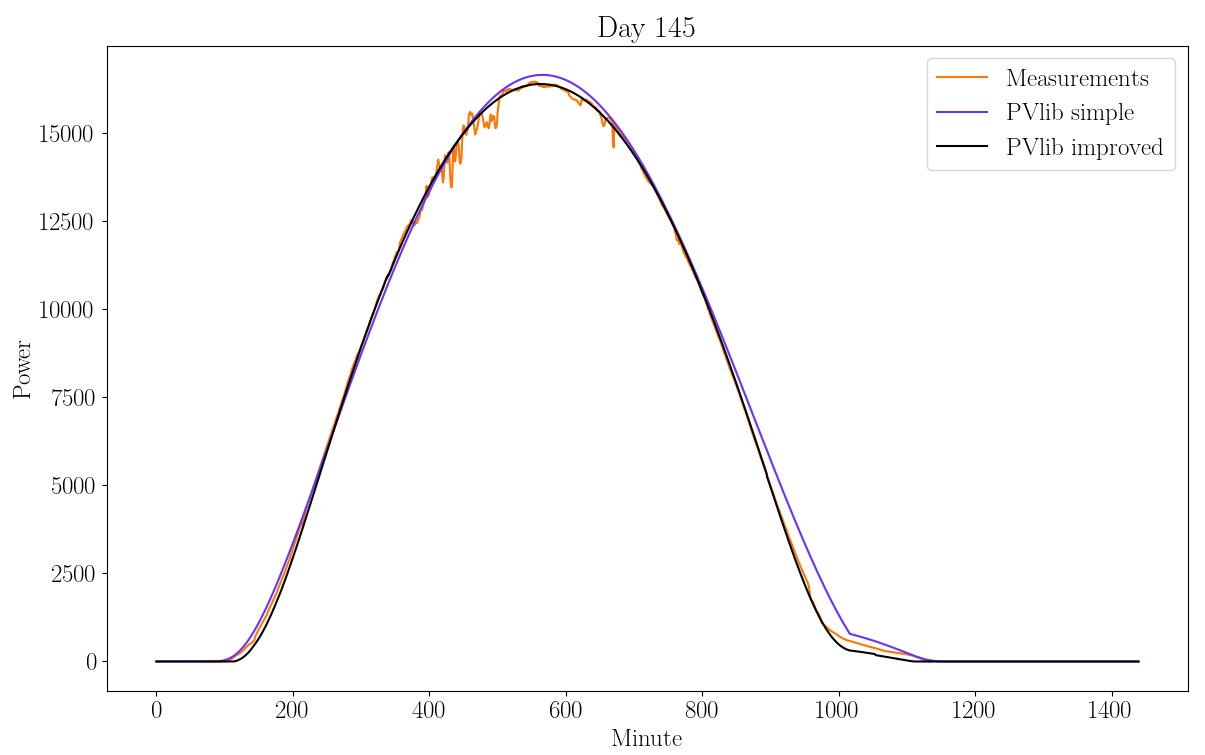
\includegraphics[width=0.99\linewidth]{pics/pvlibsimplecomplex}
\figcaption{Comparison of PVlib POA and a more accurate PV power generation model.}
\label{fig-poa_eval_simplecomplex}
\end{figure}

\noindent Figure \ref{fig-poa_eval_simplecomplex} shows that the improved PV model performs better than the simple POA-model at 1000 minutes where the AOI is high and thus reflective losses from direct irradiance are significant. And during peak production minutes where the panel temperatures are likely high enough to cause thermal losses.

The improved model would appear to be a more accurate approximation for PV generation than the POA model, but the POA model still has uses in applications where faster computation is beneficial or where only the timing of the first and last non-zero minutes matter. Which of these models is being used will be mentioned in the following chapters.

The model performance could be further tuned as inverter efficiency and other possible factors were not taken into account. However as there are only two datasets, this would increase the likelyhood of overfitting and thus the improved model is left as is.


%is near 90$^\circ$ and during peak production hours where increased temperature effects performance. This is promising but the complexcity of the model also increases the likelyhood of overfitting. Nevertheless this improved model with 2m/s wind speed, 8m elevation and 25 $^\circ$C ambient temperature and the POA model will both be used in the following chapters depending on the charasteristics of parameter estimation functions.

%\noindent Figure \ref{fig-poa_eval_single_day} show that simulations are fairly accurate but there seems to be some deviations between the simulated values and the measurements. The two significant deviations are the noise during peak power generation period and the smooth decrease in power generation during the last hours of the day. The peak power generation noise is likely to be caused by decreases in efficiency due to heat the occasional cooling from gusts of wind. The second deviation between the model and actual measurements is likely to be caused by panel reflections as the south-east orientation of the solar panels results in a high angle of incidence during the last hours of the day.

%Modeling these physical phenomena is possible to an extent if the components of plane of array irradiance are used instead of the POA values. As per Sandia National Laboratories \cite{sandia_poa}, the three components of plane of array irradiance are direct normal irradiance(DNI), global horizontal irradiance(GHI) and diffuse horizontal irradiance DHI. A physically accurate model would compute the absorbed radiation by first projecting the irradiance components to the plane of array adn the estimating the losses caused by reflections. After this is accomplished, the absorbed irradiance could be used to estimate panel temperature and power output.








